\documentclass{article}
\usepackage{tikz}
\usetikzlibrary{arrows.meta,positioning,calc,shapes.geometric}
\pagestyle{empty}
\begin{document}
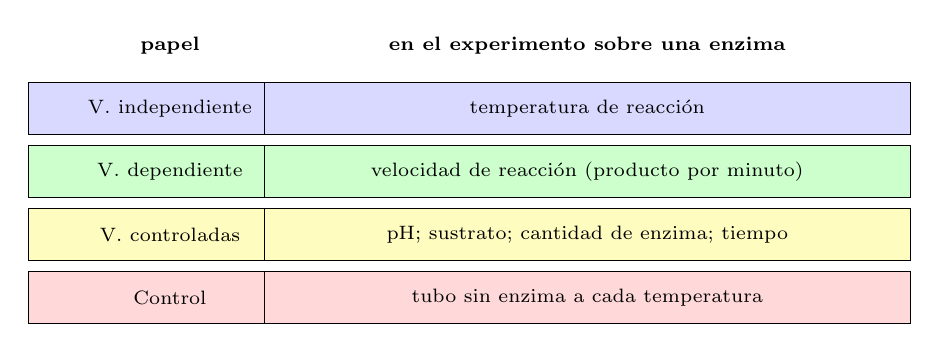
\begin{tikzpicture}
\node[font=\bfseries\scriptsize] at (2.0,3.3) {papel}; \node[font=\bfseries\scriptsize] at (7.3,3.3) {en el experimento sobre una enzima};
\node[draw, fill=blue!15, minimum width=3.6cm, minimum height=0.65cm, font=\scriptsize] at (2.0,2.5) {V. independiente}; \node[draw, fill=blue!15, minimum width=8.2cm, minimum height=0.65cm, font=\scriptsize] at (7.3,2.5) {temperatura de reacción};
\node[draw, fill=green!20, minimum width=3.6cm, minimum height=0.65cm, font=\scriptsize] at (2.0,1.7) {V. dependiente}; \node[draw, fill=green!20, minimum width=8.2cm, minimum height=0.65cm, font=\scriptsize] at (7.3,1.7) {velocidad de reacción (producto por minuto)};
\node[draw, fill=yellow!25, minimum width=3.6cm, minimum height=0.65cm, font=\scriptsize] at (2.0,0.9) {V. controladas}; \node[draw, fill=yellow!25, minimum width=8.2cm, minimum height=0.65cm, font=\scriptsize] at (7.3,0.9) {pH; sustrato; cantidad de enzima; tiempo};
\node[draw, fill=red!15, minimum width=3.6cm, minimum height=0.65cm, font=\scriptsize] at (2.0,0.1) {Control}; \node[draw, fill=red!15, minimum width=8.2cm, minimum height=0.65cm, font=\scriptsize] at (7.3,0.1) {tubo sin enzima a cada temperatura};

\end{tikzpicture}
\end{document}
